
\begin{frame}{}
    \centering \large \textbf{Word Embeddings}
\end{frame}


\begin{frame}{}
    
    \begin{definitionBlock}{Definition: Word Embedding (Words as Vectors)}
        Word embeddings are unsupervised models that capture semantic and syntactic information about words in a compact low-dimensional vector representation $\Rightarrow$ useful for reasoning about word usage and meaning (Melamud et al. 2016, p. 1).
    \end{definitionBlock}
    \vspace{-5pt}
    
    
    \begin{itemizeSpaced}{3pt}
        
        
        \pinkbox Sentence embeddings, phrase embeddings, character embeddings (for morphology)
        
        \pinkbox Can capture \textbf{vector space semantics}: can express word analogy ``man is to woman as king is to queen" with arithmetic on learned word vectors: $vector(man) - vector(woman) = vector(king) - vector(queen)$
        
    \end{itemizeSpaced}
    
    \begin{figure}[h]
    \vspace{-10pt}
    \centering
    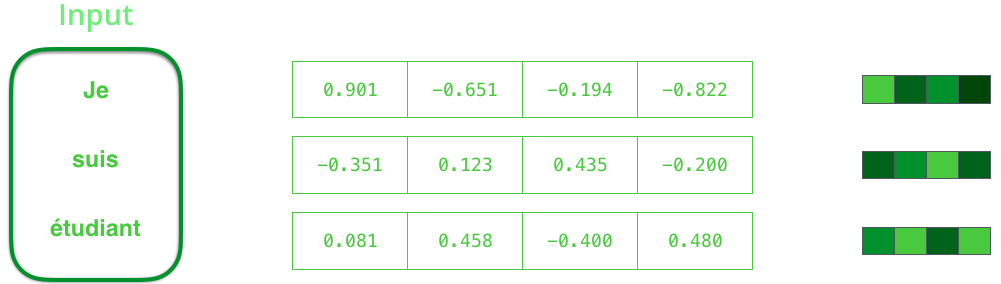
\includegraphics[width=0.8\textwidth]{imgs/example_word_embedding.png}
    \vspace{-5pt}
    \caption{\tiny \linespread{0.1} Example Word Embeddings. From \emph{Visualizing Neural Machine Translation Mechanics of Seq2Seq Models with Attention}, by Jay Alammar, 2018. \url{http://jalammar.github.io/visualizing-neural-machine-translation-mechanics-of-seq2seq-models-with-attention/}}
    \vspace{-10pt}
    \label{fig:exampleWordEmb}
    \end{figure}
    
\end{frame}



% \begin{frame}{} %{ \normalsize {\vfill\vfill Mathematically: \\How Models Make Embeddings}}
% 
%   \small\textbf{Mathematically: How Models Make Embeddings ..}
% 
% \begin{itemizeSpaced}{10pt}
%       \small
%     
%     \item a word’s conditional probability combines its \emph{embedding} and \emph{context vectors} of surrounding words, with different methods combining them differently. 
%     
%     \item Then, embeddings are fitted to text by maximizing the conditional probabilities of observed text.
%     
% \end{itemizeSpaced}
%     
% \end{frame}




\begin{frame}{What is Polysemy?}
      \small 
    
    \begin{definitionBlock}{Definition: Polysemy}
    \alert{\textbf{Polysemy}} means a word has multiple senses. 
    \end{definitionBlock}
    
    
    \begin{definitionBlock}{Definition: Distributional Hypothesis}
    \alert{\textbf{Distributional hypothesis}} is a key idea in NLP that says meaning depends on context, and words in same contexts have similar meaning (Wiedemann et al., 2019). 
    \end{definitionBlock}
\end{frame}





\begin{frame}{Static vs. Contextual Embeddings}

    \vspace{20pt}

    \begin{definitionBlock}{\footnotesize Definition: Static Embeddings}
           \alert{\textbf{Static embeddings}} (classic word vectors) assign one vector to each word, regardless of polysemy (Ethayarajh, 2019). \newline 
           
           Skip-Gram and Glove produce these ``context-free" representations because they use co-occurrence counts, not the more dynamic \textbf{language modeling} approach (Batista, 2018). 
           
    \end{definitionBlock}
    
    
    \vspace{-2pt}
    
    \begin{alertBlock}{\footnotesize Alert}
        All senses of a polysemic word are \emph{\alert{collapsed}} within a single vector representation (Ethayarajh, 2019). Confusion!  \newline 
        
        ``Plant”'s embedding would be the ``average of its different contextual semantics relating to biology, placement, manufacturing, and power generation” (Neelakantan et al., 2015).

    
    \end{alertBlock}
    
    \vspace{-2pt}
    
    \begin{definitionBlock}{\footnotesize Better: Contextual Word Embedding}
   
    A \textbf{\alert{contextual word embedding (CWE)}} captures forward and backward context using a bidirectional language model (biLM) (Antonio, 2019).   
    
    Static word embeddings are like ``look-up tables" but contextual embeddings have word type information (Smith, 2019). 
\end{definitionBlock}
      
    
\end{frame}


% 
% 
% \begin{frame}{Better: Contextual Embeddings (CWE)}
% 
% 
% \begin{definitionBlock}{Definition: Contextual Word Embedding}
%       \small
%     A \textbf{\alert{contextual word embedding (CWE)}} captures context using forward and backward history, using a bidirectional language model (biLM) (Antonio, 2019).   
%     
%     Static word embeddings are like ``look-up tables" but contextual embeddings have word type information (Smith, 2019). 
% \end{definitionBlock}
% 
% 
% \begin{itemizeSpaced}{7pt}
% 
%     \pinkbox Abandons the idea of using a fixed word sense inventory (to model polysemy) to make a vector representation for each \textbf{word type} in the vocabulary and each \textbf{word token} in a context. 
%     
%     \pinkbox Experimentally superior to static embeddings.
%     
%     \item ``sentence or context-level semantics together with word-level semantics proved to be a powerful innovation” in the NLP world (Wiedemann et al., 2019).
%     
%     
% \end{itemizeSpaced}
%     
% \end{frame}